\documentclass{article}
\usepackage{amsmath}
\usepackage{amssymb}
\usepackage{tikz}
\usetikzlibrary{automata, arrows.meta, positioning, quotes}

\begin{document}

    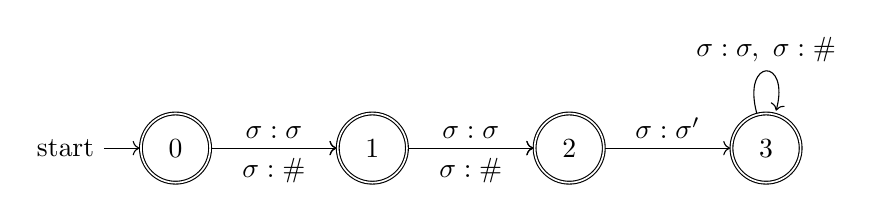
\begin{tikzpicture}[node distance = 2.5cm, on grid, auto]
    \node (q0) [state, accepting, initial] {$0$};
    \node (q1) [state, accepting, right = of q0]  {$1$};
    \node (q2) [state, accepting, right = of q1]  {$2$};
    \node (q3) [state, accepting, right = of q2] {$3$};
    \path[->] (q0) edge [above] node {$\sigma : \sigma$} (q1);
    \path[->] (q0) edge [below] node {$\sigma : \#$} (q1);

    \path[->] (q1) edge [above] node {$\sigma : \sigma$} (q2);
    \path[->] (q1) edge [below] node {$\sigma : \#$} (q2);

    \path[->] (q2) edge [above] node {$\sigma : \sigma'$} (q3);

    \path[->] (q3) edge [loop above] node {$\sigma : \sigma,~\sigma: \#$} ();
\end{tikzpicture}

\end{document}